\chapter{Fault detection in Utility Scale Photovoltaic Plants} \label{chap:chap2}


\section{Utility-Scale Photovoltaic System's Architecture}

Utility-scale photovoltaic (PV) power plants are large-scale systems connected to the electrical grid, having installed capacities ranging from kilowatts peak (kWp) to megawatts peak (MWp). These systems typically consist of many PV panels interconnected through power electronics to aggregate and inject power into the grid. The number and type of components in a PV power plant depend on the plant's scale and topology, with different configurations possible for large-scale applications, including central inverters, string inverters, and multi-string inverters \cite{lspv}. The physical installation of PV modules can include solar tracking apparatuses, such as single and dual-axis trackers \cite{Mourad2022}, which add to system complexity and change production behavior. Understanding the architecture and components of PV power plants is vital for designing, operating, and maintaining these systems, as it helps optimize their performance and reliability.

\begin{figure}[h!]
    \centering
    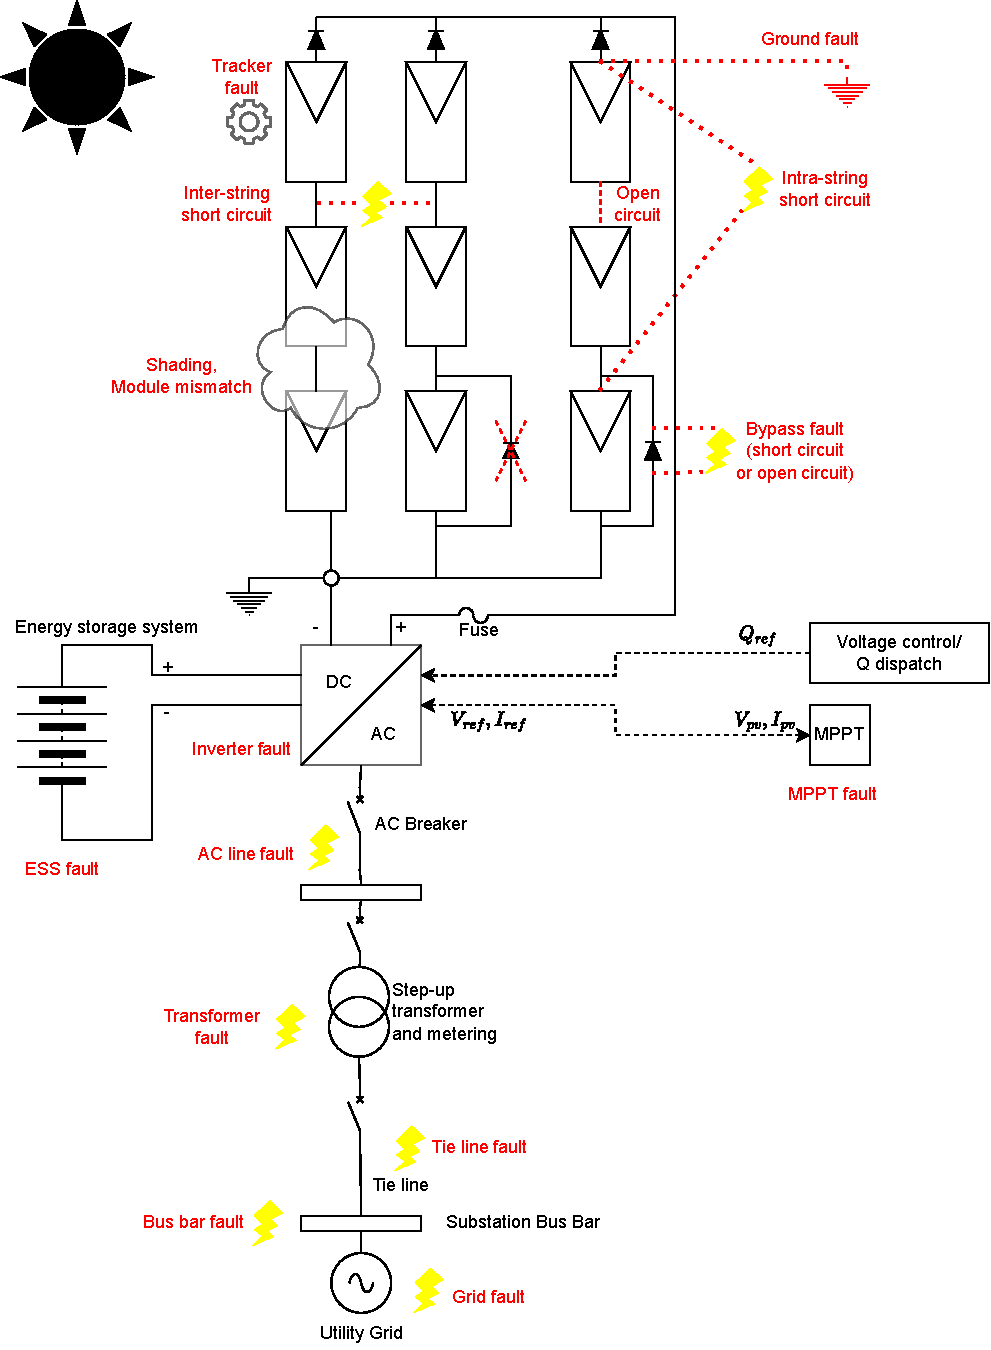
\includegraphics[width=15cm]{figures/chapter2/pvplant.drawio.pdf}
    \caption{Representation of utility-scale PV plant components and some possible faults.}
    \label{fig:topologies}
\end{figure}

Figure \ref{fig:topologies} presents a typical utility-scale PV plant architecture using the central inverter (or possibly multi-string inverter) configuration. Noticeably, many system components may fail in one or more ways, so monitoring and fault detection algorithms are essential to maintain state estimation. The main subsystems considered for anomaly detection are the following:

\begin{itemize}
    \item Solar photovoltaic panels (with or without bypass diodes).
    \item Tracking mount.
    \item Electrical cabling.
    \item Inverter(s) (mostly with Max Power Point Trackers).
    \item AC Transformer(s).
    \item Protection components (circuit breakers, fuses, surge protectors,
    etc.)
\end{itemize}

Most of these components have intrinsic variables, such as voltage and current values, that can help determine their operation states. Given that the utility grids (and the associated electricity market) integrate large-scale PV assets, some of the before-mentioned components require constant monitoring and control, achieved with adequate embedded systems and sensor infrastructure \cite{AIPV}. Since monitoring utility-scale PV assets relies on the investment and technologies employed, engineers must consider data availability when developing data-driven algorithms. Thanks to the continuous advancements in communication technologies, namely in IoT (Internet Of Things), data acquisition is becoming faster, more reliable, and more precise. Not only is this fundamental for real-time asset assessment, but it also allows better training of fault detection algorithms. However, on the industrial scale (in the order of MWp production), having sensors embedded in every PV module comes with a high economic cost. Inverters are the components that usually possess monitoring capabilities, though the grid-tie connection should also employ sensors. Consequently, these are the primary sources of information on utility-scale PV plants, with the most accurate, fast, and reliable data acquisition.

\begin{figure}[h!]
    \centering
    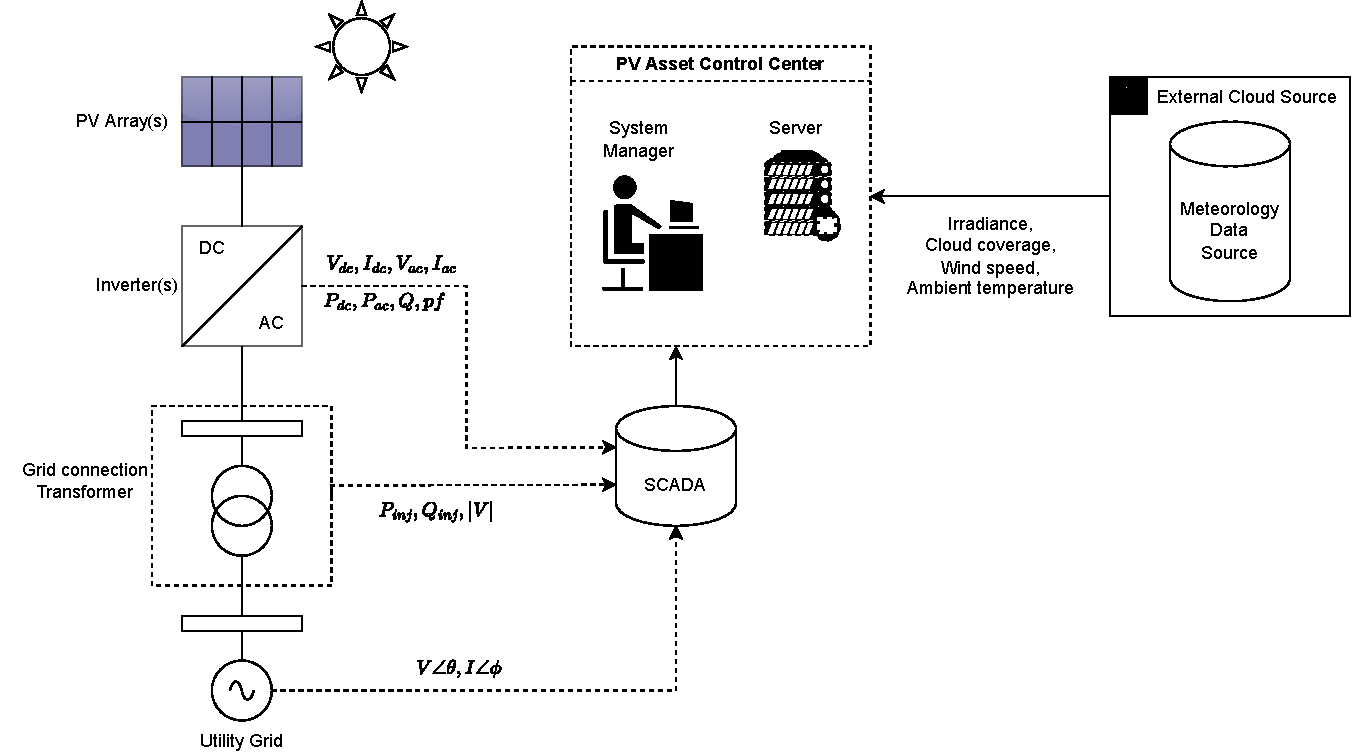
\includegraphics[width=\linewidth]{figures/chapter2/pvdata.drawio.pdf}
    \caption{Typical data flow of utility-scale PV power plants.}
    \label{fig:pvdataflow}
\end{figure}

Figure \ref{fig:pvdataflow} represents a simplified data flow representation of a grid-tied PV system's most commonly available state variables, with most of them suggested by the IEC 61724 standard \cite{iec61724}. An external meteorological data source is defined since the PV system manager usually needs climate information for (at least) forecasting purposes. The typical ranges of data acquisition periods in utility-scale PV assets are within 10 to 60 minutes.


\section{Faults in Photovoltaic Systems}

Several types of faults can occur in utility-scale photovoltaic (PV) power plants, which impact the performance and reliability of the system negatively. Unfortunately, some are very challenging to detect and protect the electrical installation against, thus requiring sophisticated detection algorithms \cite{Pillai2018}. Besides the economical price, their occurrence may even cause safety hazards, such as fires \cite{Alam2015}, thus the urgency in detecting or preventing such events early.

According to \cite{Pillai2018}, these faults can fit into three categories: electrical, mechanical, and environmental. Electrical malfunctions include short circuits, open circuits, and inverter failure, affecting the PV panels' power output and the system's overall efficiency. Mechanical faults include broken panels, damaged cables, and defective inverters, which can lead to system downtime and reduced performance (although not mentioned, solar tracker failures could also belong in this category). Environmental faults include extreme weather events, such as hail or strong winds, which can damage the PV panels and other components \cite{faults}.

The authors in \cite{Hong2022} cover a comprehensive review of most types of faults studied in the ambit of detection and classification algorithms. However, authors in \cite{Livera2019} have a more succinct fault categorization that better fits this work's scope. They categorize all the major PV system faults into either DC-side or AC-side. Figure \ref{fig:faults} represents this detailed categorization with a tree-like structure.

Although also prone to failure, most literature on fault detection and classification for photovoltaic systems does not encompass solar tracking faults: most studies cover fixed PV systems. The supervision and assessment of these subsystems' correct functioning can be sensor-based \cite{Stepanov2014} or image-based. Some authors developed fault detection methods for these apparatuses \cite{Amaral2021}, using image processing on aerial photography to determine modules' slopes. This category of failures should be better supported when developing electrical data-driven algorithms since they can significantly affect the system's efficiency.

\begin{figure}[h!]
    \centering
    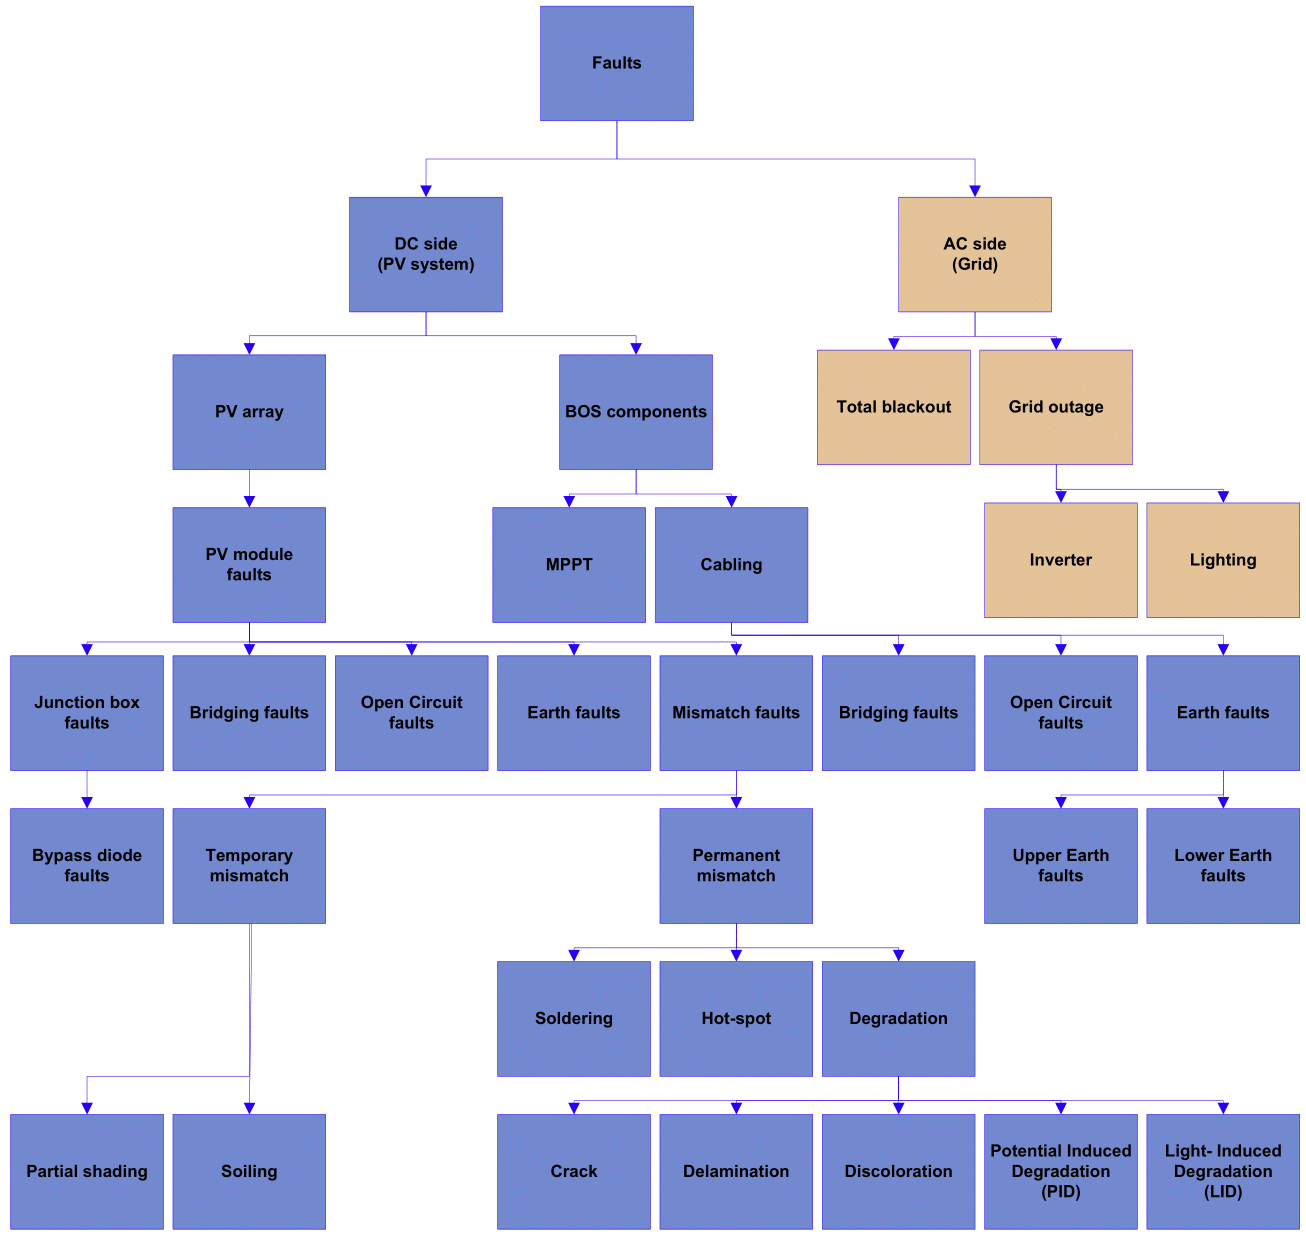
\includegraphics[width=14cm]{figures/chapter2/faults.png} \caption{"Failures in grid-connected PV systems."} Image source and copyright: \cite{Pillai2018}.
    \label{fig:faults}
\end{figure}

Throughout the literature \cite{Braun2011}, some of the most noted faults in the context of fault detection are:

\begin{itemize}
    \item Shading: partial coverage of a PV array or module, temporary or not. It might result in a Hot Spot fault.
    \item Soiling: dirt accumulation, blocking sunlight from reaching PV Cells. It might also result in a Hot Spot fault.
    \item Short circuit: either line-line or line-ground.
    \item Open circuit: connection breakage between modules.
    \item DC arc fault: electricity plasma arc formed on broken connections.
\end{itemize}

According to a 2017 survey conducted on five utility-scale PV plants in Italy \cite{Grimaccia2017}, the authors observed failure rates from <1\% to 3\% in the majority of plants and 81.8\% in the worst scenario. The high failure rate of the latter had a demonstrated cause that originated from manufacturing mistakes: snail trails. Besides this phenomenon, hot spot faults and bypass diode faults/disconnections were among the most common.

Alongside manufacturing failures, installation, planning, and other external effects can be the root cause for many of the presented faults \cite{sunny}.

\begin{figure}[h]
    \centering
    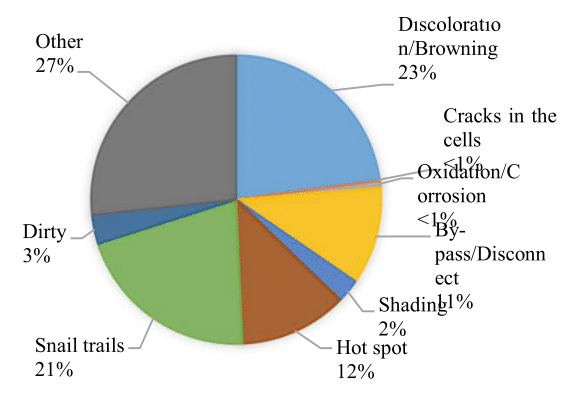
\includegraphics[width=8cm]{figures/chapter2/chartfailsurvey.png} \caption{"Circle chart related to the module defects in the 5 plants (over the total number of failures)."} Image source and copyright: \cite{Grimaccia2017}.
    \label{fig:faultchart}
\end{figure}

Having the distribution of fault types from real-life scenarios is quite helpful for formulating fault detection algorithms. It allows for better generation/selection of training data and class decisions. In Figure \ref{fig:faultchart}, it is possible to observe the failure type distribution for 24.254 inspected modules. Soiling, shading, and mechanically related failures were not as prominent, with only a group share of around 6\%. It is relevant to note that discoloration represents almost a quarter of all faults.

Although the study had a limited geographic scope, with only a few power plants diagnosed, it allows for a more realistic view of the common scenarios encountered in typical operational ground-mounted utility-scale PV power plants.

Due to the difficulty of classifying some of these faults, given their similarity on the consequent effect in the system, it will be seen in further sections that most fault detection algorithms only endeavor to classify between two to five types of reviewed faults.

\section{Modeling photovoltaic's physical/electrical behavior}

Photovoltaic cells are the fundamental components of photovoltaic panels. They are made from semiconductor materials like silicon and absorb photons that generate electric current. Their electrical behavior is characterizable using the current-voltage (I-V) equation \ref{eq:iv}. This equation, which represents a fundamental relationship governing the operation of PV cells, can be used to predict their performance under various operating conditions, such as differing solar irradiance and temperatures.

\begin{equation} \label{eq:iv}
    I = I_{ph} - I_d \times (e^{\frac{q \times (V_{pv} + I_{pv} \times R_{s})}{n \times k \times T}} - 1) - \frac{V_{pv} + I_{pv} \times R_s}{R_p}
\end{equation}

$I_{ph}$ (A) is the light-generated current;
$I_{0}$ (A) is the reverse saturation current;
$V_{pv}$ is the module's terminal voltage;
$I_{pv}$ is the module's output current;
$R_{s}$ ($\Omega$) is the series resistance;
$R_{p}$ ($\Omega$) is the shunt resistance;
$n$ (adimensional) is the diode ideality factor;
$k$ (J/K) is the Boltzman constant;
$T$ (K) is the cell temperature;
$q$ (C) is the electron charge;

For state estimation, it is crucial to accurately model PV modules' performance from the DC side of power converters. This information is vital for designing and optimizing PV power systems, as it enables predicting PV module performance under different conditions, as mentioned before. Accurate PV models are also essential for state estimation and fault detection, as they provide critical information about their health and performance, allowing for early identification of potential issues. Moreover, they can be used to optimize the control and operation of PV power systems, improving their efficiency and reliability \cite{Braun2011}.

Physical and empirical models broadly categorize the several state-of-the-art methods for modeling photovoltaic modules \cite{Braun2011}. Physical models lie on the fundamental physical principles governing PV modules' operation. They typically require detailed knowledge of the PV module's electrical and optical properties, such as its current-voltage (I-V) characteristics, spectral response, and temperature dependence. These models can accurately predict the PV module's performance under diverse operating conditions, but they may be complex and computationally intensive to implement \cite{Kumar2019}. On the other hand, empirical models are based on experimental data and are typically more straightforward to implement. However, they may not be as accurate as physical models, especially under conditions that differ significantly from those used to generate the experimental data (usually STC) \cite{Braun2011}. Some examples of state-of-the-art physical models for PV modules include the single-diode model (the five-parameter model) and the two-diode model \cite{Godina2017}. In contrast, one of the most used state-of-the-art empirical models is the Sandia model \cite{Braun2011}. Choosing a modeling method depends on the specific application and required level of accuracy and complexity; in some cases, there can be a combination of physical and empirical models.

In the case of utility-scale PV systems, detailed knowledge of the module's electrical and optical properties of empirical data may be limited, and building a model is only possible by recurring to datasheet information. A complex model that requires more detailed information may not be feasible in such cases, and a simpler model that relies on fewer input parameters is more appropriate. Given the excellent trade-off between complexity and accuracy, the single-diode model suits this use case.

\subsection{The five-parameter model}

Figure \ref{fig:onediodedraw} presents the single-diode model representation of the photovoltaic module. According to the five-parameter model, the unknown parameters are determined by fitting the model to experimental data or using data from the PV module's datasheet. The single-diode model can predict the PV module's performance under various operating conditions while maintaining reasonable accuracy. However, remembering that the single-diode model is a simplified representation of the PV module, it will have poor accuracy under certain situations compared to the more representative two-diode model \cite{Godina2017}.

\begin{figure}[H]
    \centering
    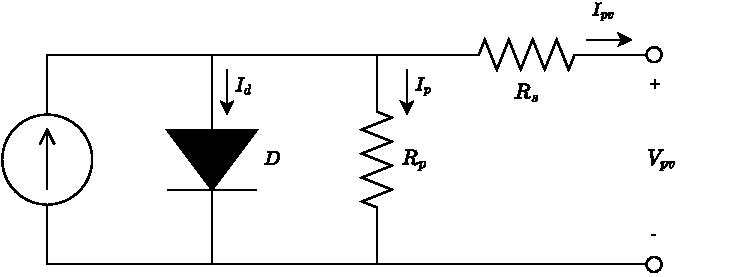
\includegraphics[width=10cm]{figures/chapter2/onediode.drawio.pdf} \caption{Single-diode model for photovoltaic modules.}
    \label{fig:onediodedraw}
\end{figure}

% \section{Characteristics of Photovoltaic Faults}
% ! fazer isto ou não?
% To better understand the effect of faults in photovoltaic systems, we review 

\section{Literature on Fault Detection and Classification for Photovoltaic Systems}

The parent field of fault detection is anomaly detection (also known as outlier detection), a highly studied subject in the scope of statistics \cite{Prasad2009}, applied in many scientific areas. Classification is also well-studied in this field, with applications in numerous scientific contexts, from medical diagnosis to airport safety \cite{classification}. Consequently, adaptations of generic tools and ad hoc methodologies have originated to aid in solving fault detection and classification problems in photovoltaics.

According to \cite{AIPV}, the tools dedicated to PV fault detection and state estimation mostly come from mathematical/statistical methodologies, machine learning , and deep learning applications. Regarding the three general problem-solving principles mentioned before, machine learning and deep learning are the most popular and successful ones for recent applications that ought to solve complex problems. However, this categorization needs to be revised, with contemporary literature suggesting many developed methodologies from different backgrounds, thoroughly reviewed in \cite{Hong2022} and \cite{Livera2019}. In \cite{Hong2022}, the authors consider two principal fault detection and classification algorithm branches: image-based and electrical-based (e.g. I-V Curve \cite{e_iv_1}\cite{e_iv_2}\cite{e_iv_3}, Power loss \cite{e_pl_1}\cite{e_pl_2}\cite{e_pl_3}\cite{e_pl_4}\cite{e_pl_5}), while \cite{Livera2019} also distinguishes numerical-based techniques (encompassing machine learning \cite{n_ann_1}\cite{n_ann_2}\cite{n_ann_3}, fuzzy logic \cite{n_f_1}\cite{n_f_2}\cite{n_f_3}, and statistical \cite{n_s_1}\cite{n_s_2}\cite{n_s_3}). Image-based refers to aerial or visual capture of the PV array by photography and thermal imaging, commonly used along with artificial intelligence algorithms for assessing the photovoltaic module's physical state. Although the contribution and importance of such methods are appreciable, this work will mainly focus on the electrical-based and numerical-based ones, as the use case of the developed tool is bound to this type of data.

Categorizing methodologies becomes fuzzy, considering that some literature mixes physical behavior models with machine learning, statistics, and signal processing. Figure \ref{fig:techniques} is an attempt to present a structure inspired by the review made by \cite{Hong2022}, \cite{Livera2019}, and this work, with a focus on the techniques more relevant for our scope. Hybrid models are ubiquitous since combining robust statistical, signal processing, ML, or DL models and PV's electrical characterization can achieve remarkable results. We conclude that various technique combinations create mixed categories of algorithms.
 
\begin{figure}[h]
    \centering
    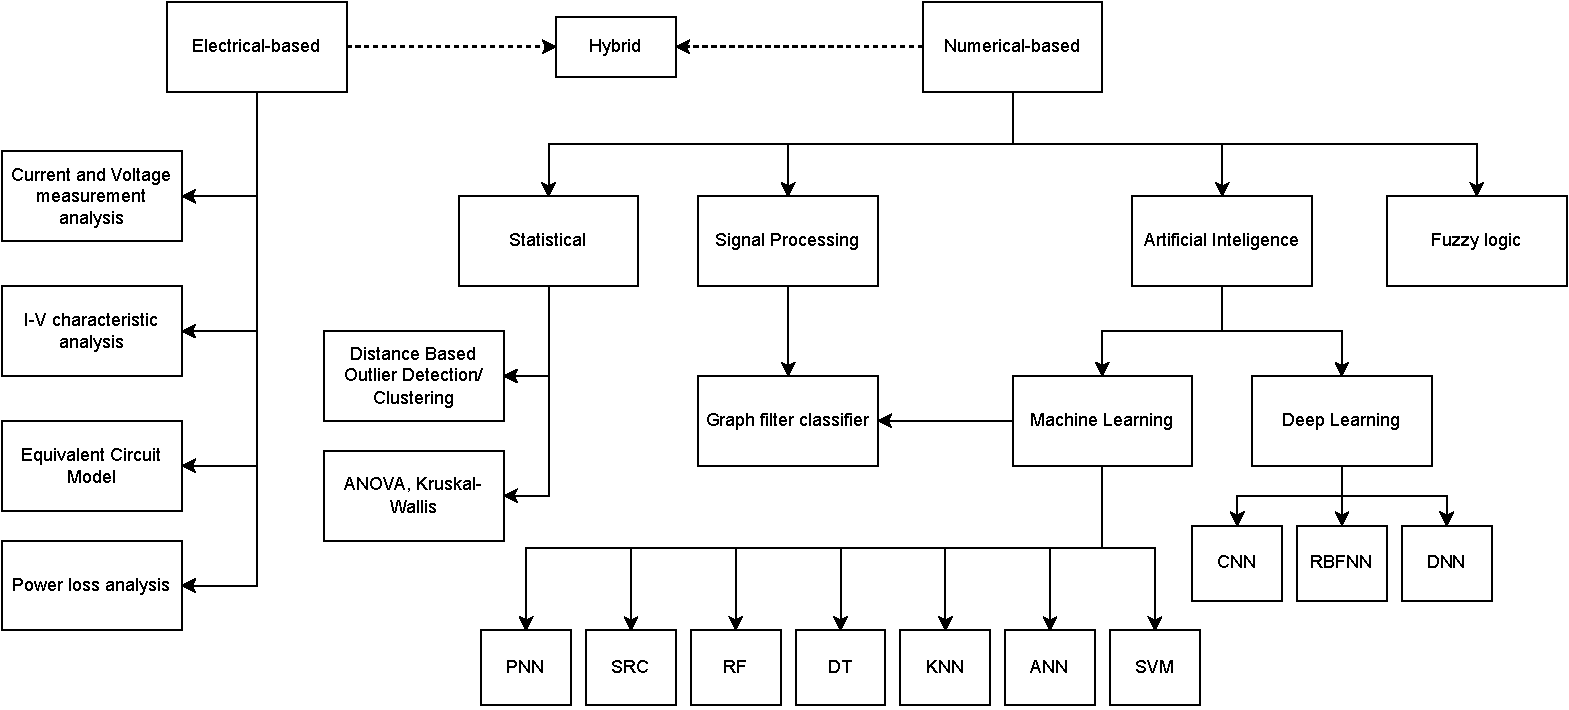
\includegraphics[width=15cm]{figures/chapter2/techniques.drawio.pdf} \caption{Representation of some of the methodologies employed in fault detection for PV systems.}
    \label{fig:techniques}
\end{figure}

Deciding which methodologies to revise is necessary to avoid wandering in the literature. The developed tool in this work must meet certain real-life constraints, such as data availability, frequency, accuracy, PV system configuration, and context. Therefore, we consider each methodology's potential (qualitative) as the proposed algorithms' adaptability to the same expected restrictions. This evaluation process confines the methodology review to emphasize the ones thought to be most capable of implementation in a real scenario. Therefore, the following sections will not cover an extensive literature review; we do not intend to repeat the works of \cite{Hong2022} and \cite{Livera2019}, only presenting interesting or adequate methodologies related to this work's scope.

\subsection{Statistical and Signal Processing Algorithms}

Statistical methodologies look into historical data to find the characteristics of how samples relate to the population (interpolation). These methodologies yield good results in case studies of PV farms that have been logging data for a considerable time, suffering in the cases that do not. Therefore, they are limited in that it is required to have curated data sets of historical significance for relevant features of the studied systems.

The literature on fault detection algorithms based on statistical and signal processing is mostly quite dated (\cite{Buddha2012}, \cite{Zhao2014}, \cite{Vergura2008}), given that more recent machine learning methods have become increasingly attractive in this matter. Nonetheless, researchers use anomaly (or outlier) detection statistical algorithms for fault detection in PV systems by identifying unusual patterns or deviations from normal behavior in the new measurements from the PV system. Distance-based methods may be adequate, such as the Euclidean, Mahalanobis, and MCD-based distances \cite{Braun2011}. Although simple, these techniques might only work for detecting outliers in the context of PV systems if they are scale-invariant (due to the different magnitude in the system's state variables) and resilient to outlier contamination (which only MCD-based distance is capable of). In \cite{Vergura2008}, the authors applied Analysis of Variance (ANOVA) and Kruskal-Wallis test for inverter failure detection, with the only downside of only being able to identify outliers in a sub-array resolution, i.e., not for specific string or module failures.

Some algorithms consider incoming data from PV systems as signals, allowing the adaptation of signal processing theory to develop ad hoc algorithms. Coming up with a relatively simple algorithm, the authors in \cite{Iles2021} propose a power-based fault detection method that only requires delayed samples of the PV array's power output and a threshold. It reasons that since the power output of PV systems cannot vary beyond a given point, considering a very short-term period (milliseconds), significant perturbations in this variable can be associated with faults. Although the simplicity and ease of implementation, it is clear that the success of this method requires feeding the algorithm with relatively high-frequency data, which would only be feasible on-site (and with specialized monitoring equipment).

In \cite{Fan2020}, the authors successfully formulated a graph signal processing algorithm for fault classification that yields increasingly better results when there is a considerable amount of labeled data, although its training is only semi-supervised. The results outperformed other standard machine learning methods for the same training data, given 30\% or more of labeled data. On another note, the data utilized came from the PVWatts \cite{Dobos2013} dataset, and the PV system is on a small scale (ASU testing facility \cite{Rao2016}) possessing a monitoring density and capability that can be considered irrealistic for utility-scale. This same data source is present in many other reviewed works.

The authors in \cite{Katoch2018} displayed another excellent use for graph theory, although not specifically for fault detection: they implemented a consensus-based distributed approach to minimize the impact of noise in acquired data from the PV array. By formulating a data propagation algorithm that resulted in measurement convergence, they achieved higher accuracy for state estimation.

With both graph theory-based algorithm proposals, this field sparks interest in its usage for the upcoming formulated methodology, given that it would be desirable to achieve an algorithm that features fault detection alongside data consensus.


\subsection{Machine Learning Algorithms} \label{subsec:machinelearning}

Machine learning is the trending way of solving increasingly complex and nonlinear problems, as neural networks (or other learning structures) can better model complex, non-trivial, and nonlinear relations between data. Still, they are as good as the training data, with many designs requiring a lot of representative learning examples to achieve good results. Their output can also be very obfuscated (depending on the technique), meaning that many methods do not allow a direct interpretation of the relationship between inputs and outputs. This "black-box" characteristic, specifically of neural networks, is considered a disadvantage. Besides, extrapolating data remains a challenge when classically using these structures. Still, they have immense applications for PV systems, from MPP (Max Power Point) estimation to power forecasting, soiling, and fault prediction.

In \cite{Kumari2022}, the authors utilize an ANN to classify short circuit and hot spot faults. This algorithm achieved an outstanding 98.4\% classification accuracy, yet the data originated from \textit{MatLab/Simulink} simulations and only considered two classes of faults. Because the inputs were the variation of voltage and current ($\frac{dV}{dt},\frac{dI}{dt}$), the algorithm required data sampling with relatively high frequency (>5Hz). This work will not regard such methodologies as background for the upcoming tool since requiring high-frequency simulated data while covering only two fault types is quite far from a real utility-scale PV system scenario.

The trend of utilizing simulated data (sometimes without even added noise) has been a target of criticism in \cite{Aziz2020}. Accordingly, this work also emphasizes that the literature shows many proposed ML (and other types of) techniques that fall into this concept, which makes selecting appropriate methodologies to base future work on a challenging task.

The proposed ANN solution in \cite{Rao2019} is remarkable by the diversity of fault classification achieved: STC, short circuit, varying temperature, partial shading, complete shading, degraded modules, ground fault, and arc fault. It presents one of the most accurate fault class coverage in the group of literature that utilizes synthetic noiseless data. Hence, the cyber-physical conceptualization and data preprocessing (clustering) demonstrated can be admired, but not forgetting that validation data came from a relatively unrealistic setting. 

In \cite{Rao2021}, there is a captivating proposal of utilizing an autoencoder and pruned neural network to separate the tasks of detecting and classifying faults, which resulted in one of the most performant ML approaches in the literature. The algorithm classifies five states: degraded, shaded, soiled, short circuit, and STC, utilizing nine inputs representing voltage, current, power, and irradiance available from the MPPT, datasheet, or meteorological sources. While the neural network pruning adds complexity, it resulted in a better generalized and lighter-weight trained model suitable for faster detection times. Even though using data from a small-scale PV system, the presented algorithm and its assumptions may make it possible to adapt and implement in an industrial scenario.

Regarding performance, the work in \cite{Kilic2020} proposes a sparse representation classifier (SRC) that evaluates if the system has line-to-line or line-to-ground faults for varying operating conditions. Although a drop in accuracy occurred for extreme circumstances, it is impressive that the algorithm identifies faults in such varied operating conditions: 10 to 50 degrees ambient temperature, 200 to 1000 $W/m^2$ irradiance, 10 to 60 \% of mismatch, and 0 to 25 $\Omega$ of fault resistance. The feature extraction step was also very impressive, which could be a determining factor in the method's performance. Unfortunately, this work also does not validate results with experimental data and only uses simulation as a source. However, the demonstrated computational performance, both in terms of training cost and utilization speed, its usage without the need for training for parameter tuning, the straightforward implementation, and consistent convergence, suggests the potential for this alternative in the face of other ML methodologies. The authors also emphasize that sparse representation might be utilized alongside different learning algorithms for classification, opening the door to many possible future implementations.

Authors in \cite{Uehara2021} made an exciting yet far-fetched proposal, developing a quantum neural network (QNN) for PV fault classification. They trained the QNN to predict only two scenarios: faulty or standard, but required up to four training days, resulting in 93.89\% accuracy. For comparison, the classical ANN took twenty seconds to train and achieved 95.39\% accuracy. Although the methodology showcases the potential of quantum computing for this field, its preliminary results still distance itself from the traditional methods.

An abundance of ML methods has been tested and reviewed in this field (\cite{Hong2022},\cite{Livera2019}), utilizing structures such as SVM, KNN, and RF. Nonetheless, the results of \cite{Rao2021}-\cite{Kilic2020} sparked the most interest in this work's scope.

\subsection{Deep Learning Algorithms}

Deep learning branches from machine learning, with the term "deep" referring to amplified machine learning structures that ought to understand data patterns through more complex and intertwined artificial neuron connections. A simple example of a deep learning model would be the design of an artificial neural network with multiple hidden layers (DNN), with the intuition that each of these "extra" layers achieves feature/pattern recognition in a cascade. Other DL structures include the LSTM, CNN, and RBFNN. They have been explored alongside classical machine learning techniques for PV fault detection, although the known disadvantage is a usually high computational cost and relatively tricky implementation. The typical application of these techniques is in image-based solutions \cite{termoreview} since they require classification based on 2D data from various image acquisition equipment \cite{termo}, \cite{dlpv}. Given the 1D characteristic of raw electrical data, little literature considers these techniques for fault detection, as it implies an extra step of increasing dimensionality. However, there are some promising results in doing so \cite{Aziz2020}.

In \cite{Aziz2020}, not only is a DL technique presented for fault detection and classification, but there is also the best attempt at comparative evaluation against other methodologies. As mentioned, much of the literature presents results solely based on particular datasets comprising simulated noiseless data, invalidating any significant quantitative comparison.

Authors in \cite{Krizhevsky2012} use a CNN model based on the pre-trained AlexNet for classification and feature extraction, allied with a classical ML model also for classification. The classified faults were arc fault, partial shading, open circuit, and short circuit. While the experiments utilized simulation data, adding noise and an abundance of heterogenous operating conditions better resembled a real scenario. Considering the same noisy data, other tested methodologies present 22-70\% average accuracies, with the proposed fine-tuned AlexNet CNN reaching a maximum of 70.45\%. This work presents one of the best benchmarks in the literature, with decent coverage of other state-of-the-art ML and DL algorithms, while demonstrating the most realistic results and a sophisticated methodology proposal.

Table \ref{tab:comparelit} summarizes the comparison between four of the most inspiring reviewed proposals from the literature mentioned in this work.

\begin{table}[h]
    \centering
    \caption{Comparison of literature that inspired this work.}
    \label{tab:comparelit}
    \resizebox{\textwidth}{!}{%
    \begin{tabular}{|l|l|l|l|l|c|c|l|l|}
    \hline
    \multicolumn{1}{|c|}{\textbf{\begin{tabular}[c]{@{}c@{}}Reference\\ and year\end{tabular}}} &
      \multicolumn{1}{c|}{\textbf{\begin{tabular}[c]{@{}c@{}}Data\\ Source\end{tabular}}} &
      \multicolumn{1}{c|}{\textbf{Inputs}} &
      \multicolumn{1}{c|}{\textbf{\begin{tabular}[c]{@{}c@{}}Proposed\\ methodology\end{tabular}}} &
      \multicolumn{1}{c|}{\textbf{\begin{tabular}[c]{@{}c@{}}Classified Faults\\ (alongside STC)\end{tabular}}} &
      \textbf{\begin{tabular}[c]{@{}c@{}}Validation\\ data\\ realism\end{tabular}} &
      \textbf{\begin{tabular}[c]{@{}c@{}}Computational\\ cost\end{tabular}} &
      \multicolumn{1}{c|}{\textbf{Notes}} &
      \multicolumn{1}{c|}{\textbf{Drawbacks}} \\ \hline
    \begin{tabular}[c]{@{}l@{}}\cite{Aziz2020}\\ \\ 2020\end{tabular} &
      \begin{tabular}[c]{@{}l@{}}Simulated \\ PV System,\\ added noise\end{tabular} &
      \begin{tabular}[c]{@{}l@{}}Irradiance,\\ Temperature,\\ Short circuit current,\\ Open circuit voltage,\\ PV current,\\ MPP current,\\ MPP voltage,\\ MPP power.\\ Boost converter\\ Maximum current,\\ Voltage and power.\end{tabular} &
      \begin{tabular}[c]{@{}l@{}}Pre-trained\\ CNN (AlexNet)\\ for feature extraction\\ and classification\end{tabular} &
      \begin{tabular}[c]{@{}l@{}}Arc fault,\\ Partial shading,\\ Fault\\ during\\ partial shading,\\ Open circuit, \\ Line to line SC\end{tabular} &
      Moderate &
      High &
      \begin{tabular}[c]{@{}l@{}}Resilient against noisy data.\\ Outperforms classical ML\\ methodologies.\end{tabular} &
      \begin{tabular}[c]{@{}l@{}}Requires data samples\\ from the MPPT\\ boost converter.\end{tabular} \\ \hline
    \begin{tabular}[c]{@{}l@{}}\cite{Kilic2020}\\ \\ 2020\end{tabular} &
      \begin{tabular}[c]{@{}l@{}}Simulated\\ PV System,\\ no added noise\end{tabular} &
      \begin{tabular}[c]{@{}l@{}}MPP voltage, \\ MPP current,\\ Short circuit current,\\ Open circuit voltage,\\ Irradiance\end{tabular} &
      \begin{tabular}[c]{@{}l@{}}Sparse\\ representation\\ classifier\end{tabular} &
      \begin{tabular}[c]{@{}l@{}}Line to line SC\\ Line to ground SC\end{tabular} &
      Low &
      Low &
      \begin{tabular}[c]{@{}l@{}}Very fast learning speed compared to\\ classical ML structures.\\ Straightforward implementation.\\ Good feature extraction process.\end{tabular} &
      \begin{tabular}[c]{@{}l@{}}Validation data\\ was very idealistic.\\ Only classifies line to line\\ and line to ground faults.\end{tabular} \\ \hline
    \begin{tabular}[c]{@{}l@{}}\cite{Fan2020}\\ \\ 2020\end{tabular} &
      \multirow{2}{*}{\begin{tabular}[c]{@{}l@{}}PVWatts\\ dataset\end{tabular}} &
      \multirow{2}{*}{\begin{tabular}[c]{@{}l@{}}MPP voltage,\\ MPP current,\\ Short circuit current,\\ Open circuit voltage,\\ Irradiance, Fill factor,\\ Temperature,\\ Gamma ratio,\\ Maximum power\end{tabular}} &
      Graph signal processing &
      \multirow{2}{*}{\begin{tabular}[c]{@{}l@{}}Shading\\ Degraded modules\\ Soiling\\ Short circuit\end{tabular}} &
      \multirow{2}{*}{High} &
      Low &
      \begin{tabular}[c]{@{}l@{}}Semi-supervised,\\ allows usage of\\ unlabeled data for training.\\ Better accuracy relatively to other\\ ML methods for less labeled data. \\ Low training cost.\end{tabular} &
      - \\ \cline{1-1} \cline{4-4} \cline{7-9} 
    \begin{tabular}[c]{@{}l@{}}\cite{Rao2021}\\ \\ 2021\end{tabular} &
       &
       &
      \begin{tabular}[c]{@{}l@{}}Autoencoder for detection\\ and pruned neural network\\ for classification\end{tabular} &
       &
       &
      Medium &
      \begin{tabular}[c]{@{}l@{}}Separate the task of\\ detection from classification,\\ allowing for other combinations.\\ Good performance method\\ considering the\\ algorithms complexity.\\ Pruning creates an\\ ANN less prone to overfitting.\end{tabular} &
      \begin{tabular}[c]{@{}l@{}}Requires more complex\\ training phase, for two\\ different networks, and\\ utilizing a dropout\\ algorithm for pruning.\end{tabular} \\ \hline
    \end{tabular}%
    }
    \end{table}


\section{Cell Networks}

Although researchers commonly use machine learning and statistical methods for fault detection, the unique topology of photovoltaic (PV) systems presents a compelling case for a distributed approach. PV systems often comprise interconnected components, such as solar panels and inverters, distributed across a wide geographical area. The decentralized nature of these systems poses challenges for centralized fault detection algorithms. However, by leveraging the network-like structure of PV systems, a distributed approach can take advantage of the inherent connectivity and communication between components. This distributed approach can enable localized fault detection and diagnosis, allowing more accurate and efficient identification of faults within the PV system.

Weighted coupled cell networks (WCCN) are mathematical models that study complex dynamical systems composed of interconnected cells (or units) \cite{Aguiar2010} \cite{Aguiar2020}. In these networks, each cell interacts with its neighboring cells through weighted connections, where the weights represent the strengths or influence of the interactions. The weights can be positive or negative, indicating the nature of the coupling, whether it is excitatory or inhibitory. Differential equations or discrete-time maps often describe the dynamics of the cells, and the weights determine the coupling strength between the cells. By adjusting the weights, researchers can investigate how different connectivity patterns impact the overall behavior of the network, including synchronization, oscillations, and pattern formation. Weighted coupled cell networks have applications in various fields, such as neuroscience, physics, biology, and social sciences, providing insights into interconnected systems' emergent behavior and collective dynamics. Studying these networks allows researchers to gain a deeper understanding of complex phenomena and develop strategies for controllin g and manipulating network dynamics in real-world systems.

Electrical systems can be classified as coupled dynamical systems, as defined by authors in \cite{Aguiar2010}. These systems, characterized by interconnected components and signal propagation, can be modeled as weighted coupled cell networks. These networks provide a framework for analyzing synchronization, stability, and the emergence of complex patterns. Moreover, they offer opportunities for optimizing system performance by adjusting weights to enhance power transmission, energy efficiency, and signal quality. Additionally, weighted coupled cell networks have the potential to contribute to fault diagnosis and control strategies, enabling the identification of system faults.

Authors in \cite{Ho2015} present the practical usage of cell networks to represent entire communication networks. They formulate a methodology for minimizing energy consumption throughout the network, with the premise that cell coupling occurs due to the mutual interference of amplifiers.

Using the concept of weighted coupled cell networks as inspiration, developing a method for detecting faults in PV systems through a cellular network representation has great potential. This approach can capture interactions and dependencies within the PV system by assigning weights to interconnected components and analyzing system dynamics. Fault detection algorithms could then monitor individual cells for abnormalities.

\section{Proposed method's scope}


While classical fault detection resides in the synchronous and direct evaluation of state and climate variables, realistic industrial scenarios can have data from various types, sources, and acquisition rates. Previously (Section \ref{sec:cellnets}), we also pointed out the topological differences and the potential advantage of facing this problem by respecting the PV system's distributed nature.
It is also important to realize that monitoring equipment can register erroneous information, and current communication technology is also susceptible to delays and data loss, aggravating the troubles for non-robust centralized algorithms.

To reflect all the issues of tangible PV assets with kW to MW of power, the authors in \cite{Livera2022} made excellent failure diagnosis and loss estimation algorithms tailored for industrial-scale PV farms. In such work, it is noticeable how different the algorithms are from classical, less "practical" approaches. Their approach inspires this work to stray from standard practices and formulate another methodology with the same orientation for practical implementation in large-scale PV.
Recent developments in the intelligent composition of deep learning structures aligned with graph theory spark some interest in their application to this field, such as the new deep learning technique named Cell Complex Neural Networks \cite{Hajij2020}. The motivation for choosing such a structure comes from its data propagation and consensus capability. The propagation techniques utilized in a CXN appeal to graph theory, dividing a system into other subsystems and components (nodes, also called cells in \cite{Hajij2020}) that share information. However, directly applying this structure might not be feasible or grant better results in fault detection. Alongside WCCNs, this also inspired this work's approach.

We intend to approach PV fault detection through a distributed and cellular methodology. This approach is challenging to categorize against what we currently find in the literature. It aims at an asynchronous and online application, which differs from most current methods. We also desire to convey a benchmark utilizing data from tangible utility-scale PV assets, allowing its assessment in a realistic scenario.
